\subsection{Feature description}
\label{sec:feature_description}

Once we have detected a keypoint $(x^*,y^*,\sigma^*)$ we need to describe it.
Let's call $f[x,y]*g[x,y,\sigma^*]=f[x,y\sigma^*]$ and a patch $P$ centered in $(x^*,y^*)$ with size $d$
$P[x,y,d]=\{[x,y]:dist_\infty((x,y),(x^*,y^*))\le d\}$

We can write a gradient as magnitude and orientation:
\[
    \nabla f[x,y,\sigma^*]=\begin{cases}
        ||\nabla f[x,y,\sigma^*]|| \\
        \alpha(\nabla f[x,y,\sigma^*])
    \end{cases}
\]

We take the patch centered in a keypoint with $d=2\lambda_1\sigma^*$ (typically $\lambda_1=4.5$)
and we have to find the "most important" gradient orientation.
We call this angle $\theta^*$.
To find this angle, for every pixel in the patch we compute the gradient and then
we build the orientation histogram.
We use $K_1=36$ bins and we divide the $[0,2\pi]$ range in $K_1$ bins.
We assign the bin $R=\left\lfloor \frac{K_1}{2\pi} \alpha(\nabla f[x,y,\sigma^*]) \right\rfloor$
to every pixel in the patch and we increment the corresponding bin in the histogram proportionally
to the magnitude of the gradient in that point.

\begin{figure}[H]
    \centering
    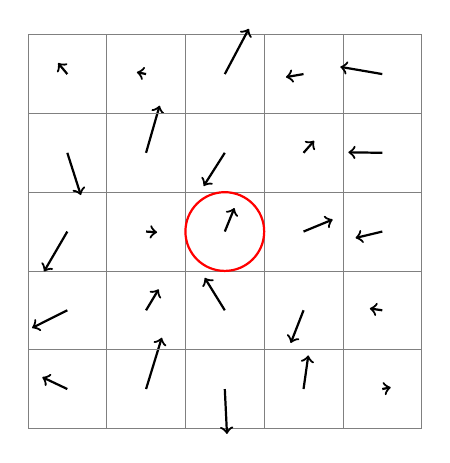
\begin{tikzpicture}
        \foreach \x in {0,1,...,4} {
            \foreach \y in {0,1,...,4} {
                \pgfmathsetmacro\angle{rand*360}
                \pgfmathsetmacro\length{0.4 + rand*0.3}
                \draw[gray, very thin] (\x, \y) rectangle (\x+1, \y+1);
                \draw[->, thick] (\x+0.5, \y+0.5) -- ++(\angle:\length);
            }
        }
        \draw[red, thick] (2.5, 2.5) circle (0.5);
    \end{tikzpicture}
    \caption{Patch with gradient arrows for each pixel. The red circle indicates the keypoint.}
    \label{fig:patch_gradients}
\end{figure}

\begin{figure}[H]
    \centering
    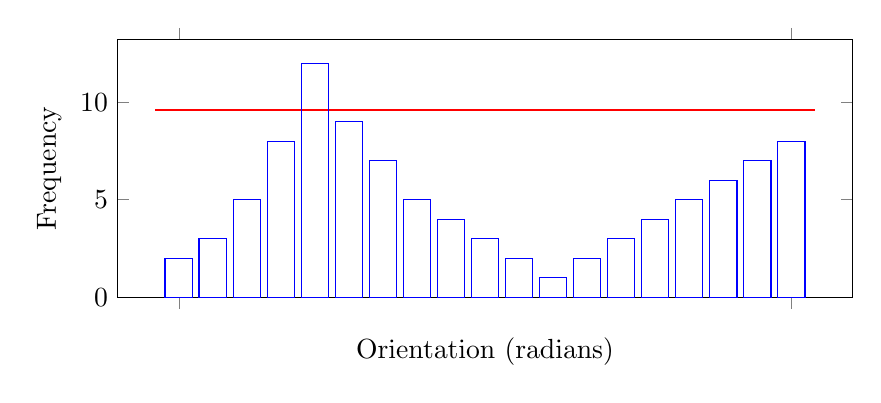
\begin{tikzpicture}
        \begin{axis}[
            ybar,
            xtick=data,
            x tick label style={rotate=90, anchor=east},
            ymin=0,
            ylabel={Frequency},
            xlabel={Orientation (radians)},
            width=0.9\textwidth,
            height=0.4\textwidth,
            xticklabels={},
        ]
        \addplot[red, line legend, sharp plot, nodes near coords={},
            update limits=false,shorten >=-3mm,shorten <=-3mm] 
        coordinates {(0,9.6) (18,9.6)};
        \addplot[blue] coordinates { 
            (0, 2) (1, 3) (2, 5) (3, 8) 
            (4, 12) (5, 9) (6, 7) 
            (7, 5) (8, 4) (9, 3) 
            (10, 2) (11, 1) (12, 2) 
            (13, 3) (14, 4) (15, 5) 
            (16, 6) (17, 7) (18, 8)
        };
        \end{axis}
    \end{tikzpicture}
    \caption{Orientation histogram for the gradients in the patch. The red dashed line indicates the threshold at 0.8 times the maximum bin value.}
    \label{fig:orientation_histogram}
\end{figure}

\begin{figure}[H]
    \centering
    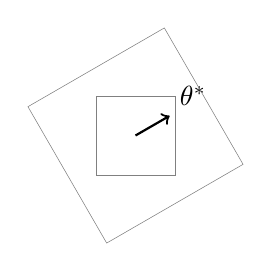
\begin{tikzpicture}
        % Draw the original patch
        \draw[gray, very thin] (0, 0) rectangle (1, 1);
        \draw[->, thick] (0.5, 0.5) -- ++(30:0.5) node[anchor=south west] {$\theta^*$};
        
        % Draw the rotated patch
        \begin{scope}[rotate around={30:(0.5,0.5)}]
            \draw[gray, very thin] (-0.5, -0.5) rectangle (1.5, 1.5);
        \end{scope}
    \end{tikzpicture}
    \caption{Original patch and rotated patch.}
    \label{fig:rotated_patch}
\end{figure}

If the new patch falls outside the image we \textbf{discard} the keypoint.

We select all the bins that are greater than 0.8 times the maximum value in the histogram.
We treat each of these bins as an individual keypoint and patch.

For each of these bins we rotate the patch such that the angle $\theta^*$ points to
the right. Actually this is done by counter-rotating the image by $\theta^*$.
Once we have counter-rotated the image we select a new patch of size $d=2\lambda_2\sigma^*$
(typically $\lambda_2=6$) on the new rotated image.

We call this new patch $P_{desc}$ and divide it into $N=4$ subpatches. For each subpatch we
compute a new orientation histogram using the gradient $\nabla f[\hat{x},\hat{y},\lambda_2\sigma^*]$ (where
the hat indicates the coordinates in the rotated image).
We use $K_2=8$ bins for this histogram. We obtain $N^2K_2$ values.

We call the vector of all these values the \textbf{feature vector} $\psi$.
This feature vector will be sparse, with most of the values being zero.

We clamp the values of the feature vector such that they are in the range $[0,0.2||\psi||]$
and we normalize the vector such that $||\psi||=512$.
Each component is quantized in 8 bits.
In this way the vector will be 128B.
The resulting vector is called \textbf{SIFT feature descriptor} corresponding to the keypoint
$(x^*,y^*)$